%

\documentclass{article}

\usepackage{fancyhdr} % Required for custom headers
\usepackage{extramarks} % Required for headers and footers
\usepackage{graphicx} % Required to insert images
\usepackage{enumerate}
\usepackage{amsmath}
\usepackage{bbold}

% Margins
\topmargin=-0.45in
\evensidemargin=0in
\oddsidemargin=0in
\textwidth=6.5in
\textheight=9.0in
\headsep=0.25in 

\linespread{1.1} % Line spacing

% Set up the header and footer
\pagestyle{fancy}
\lhead{Linear Algebra with Application\\
to Engineering Computation}
\chead{}
\rhead{CME 200/ME300A\\
M. Gerritsen\\
Fall 2013}
\headheight = 40pt



%th in the exponent (e.g. when writing ith, instead use i$\eth$)
\newcommand{\eth}{^{\text{th}}}


\newcommand{\R}{\mathbb{R}}

%short-cuts for Greek letters
\newcommand{\al}{\alpha}
\newcommand{\dlt}{\delta}
\newcommand{\eps}{\epsilon}

%times (cross-product)
\newcommand{\x}{\times}
%inverse
\newcommand{\inv}{^{-1}}
%cond
\newcommand{\cond}{\mathrm{cond}}
%trace
\newcommand{\trace}{\mathrm{trace}}

\newcommand{\twith}{\text{ with }}
\newcommand{\tand}{\text{ and }}
\newcommand{\tfor}{\text{ for }}
\newcommand{\tor}{\text{ or }}

\newcommand{\ip}{_{i+1}}
\newcommand{\im}{_{i-1}}

\newcommand{\half}{\frac{1}{2}}
\newcommand{\oneby}[1]{\frac{1}{#1}}
\newcommand{\overto}[1]{\overset{#1}{\longrightarrow}} 
 
\renewcommand\headrulewidth{0.4pt} % Size of the header rule
\renewcommand\footrulewidth{0.4pt} % Size of the footer rule

\setlength\parindent{0pt} % Removes all indentation from paragraphs

%----------------------------------------------------------------------------------------
%       DOCUMENT STRUCTURE COMMANDS
%       Skip this unless you know what you're doing
%----------------------------------------------------------------------------------------

% Header and footer for when a page split occurs within a problem environment
\newcommand{\enterProblemHeader}[1]{
\nobreak\extramarks{#1}{#1 continued on next page\ldots}\nobreak
\nobreak\extramarks{#1 (continued)}{#1 continued on next page\ldots}\nobreak
}

% Header and footer for when a page split occurs between problem environments
\newcommand{\exitProblemHeader}[1]{
\nobreak\extramarks{#1 (continued)}{#1 continued on next page\ldots}\nobreak
\nobreak\extramarks{#1}{}\nobreak
}

\setcounter{secnumdepth}{0} % Removes default section numbers
\newcounter{homeworkProblemCounter} % Creates a counter to keep track of the number of problems

\newcommand{\homeworkProblemName}{}
\newenvironment{homeworkProblem}[1][Problem \arabic{homeworkProblemCounter}]{ % Makes a new environment called homeworkProblem which takes 1 argument (custom name) but the default is "Problem #"
\stepcounter{homeworkProblemCounter} % Increase counter for number of problems
\renewcommand{\homeworkProblemName}{#1} % Assign \homeworkProblemName the name of the problem
\section{\homeworkProblemName} % Make a section in the document with the custom problem count
\enterProblemHeader{\homeworkProblemName} % Header and footer within the environment
}{
\exitProblemHeader{\homeworkProblemName} % Header and footer after the environment
}
\newcommand\overmat[2]{%
  \makebox[0pt][l]{$\smash{\overbrace{\phantom{%
    \begin{matrix}#2\end{matrix}}}^{\text{$#1$}}}$}#2}

\newcommand{\problemAnswer}[1]{ % Defines the problem answer command with the content as the only argument
\noindent\framebox[\columnwidth][c]{\begin{minipage}{0.98\columnwidth}#1\end{minipage}} % Makes the box around the problem answer and puts the content inside
}

\title{Assignment 6}
\date{Issued: November 6, 2013}
\author{Due: November 13, in class\\
No late assignments accepted}

%----------------------------------------------------------------------------------------

\begin{document}

\maketitle
\thispagestyle{fancy}
\textbf{Important:}
\begin{itemize}
\item Give complete answers: Do not only give mathematical formulae, but explain what you are doing. Conversely, do not leave out critical intermediate steps in mathematical derivations.
\item Write your \textbf{name} as well as your \textbf{Sunet ID} on your assignment. \textbf{Please staple pages together.} Points will be docked otherwise.
\item Questions preceded by  $\star$  are harder and/or more involved.
\end{itemize}


% Problem 1
\begin{homeworkProblem}

PageRank algorithms revisited (65 pts) Note: For this problem, please refer back to Assignment 5. The solutions will help you in coding your PageRank algorithm.

Recall the linear system for Page Rank:
$$ (I - \alpha P) \vec{x} = \vec{v}$$
where $\alpha$ is the fraction of a page�s rank that it propagates to neighbors at each step and $\vec{v}$ the initial rank
we give to each page. In our problem, we set $\alpha = 0.85$ and the entries of $\vec{v}$ to be $\vec{v}_i$ = $\frac{1}{n}$, with $n$ the total
number of pages in our network.

The PageRank calculation need not only be used for the internet! In fact, PageRank can be calculated for
nodes on any connected graph representing any abstraction. For this problem, we will consider a graph of
movies connected by links if they share at least one common actor. For this purpose, we provide a matlab date file $\texttt{movies.mat}$ that can be downloaded from the Materials $->$ Assignments2013 folder on Coursework.
Place this file in a local directory accessible in matlab and type $\texttt{clear all; load movies.mat}$. If you look
in the workspace, you should have a collection of new variables, defined as follows:



\begin{itemize}
\item \texttt{links} : rows are (movie, person) pairs (e.g., for \texttt{links(1,:)} equal to [779,20278] means that actor
personName{20278} was in movie movieName{779}) (James �Jimmy� Stewart in the movie Rope)
\item \texttt{movieIMDbID} : the IMDb IDs of each movie
\item \texttt{movieName} : the name of each movie
\item \texttt{movieRating} : the average IMDb rating of people who have rated this movie online
\item \texttt{movieVotes} : the number of people who have rated this movie on IMDb
\item \texttt{movieYear} : the year in which this movie was released
\item \texttt{personIMDBID} : the IMDB IDs of each actor/actress
\item \texttt{personName} : the name of each actor/actress
\end{itemize}
None of these are the proper PageRank matrix $P$.
\begin{enumerate}[(a)]
\item  (20 points)
Let $C$ be the $m \times n$ matrix defined by $C_{ij} = 1$ if movie i contains actor/actress j. Let $B$ be the $m \times m $ matrix where $B_{ij}$ is the number of actors starring in both movie i and movie j.
\begin{enumerate}[(i)]
\item Show how to calculate $B$ from $C$.
\item Show how to calculate the PageRank matrix $P$ from $B$: (Hint: it may help to construct a small graph of movies and actors (need not be based on real data) and to actually construct these individual matrices). Remember that movie $i$ and movie $j$ sharing  at least one actor counts as one link from movie $i$ to movie $j$.     
\end{enumerate}
\item (10 points)
Using matlab, construct the PageRank matrix $P$. DO NOT PRINT THIS MATRIX OUT. Instead, submit the sparsity plot of $P$ using the command $\texttt{spy(P)}$. Use sparse matrix commands to assist you; otherwise, matlab may be temperamental.
\item (10 points)
Compute the PageRank vector $\vec{x}$ of the movies in this graph and normalize this quantity so $||\vec{x}||_1 = 1$. List the
PageRank values and titles of the movies with the five highest PageRank values.
\item (15 points)
Compute the PageRank vector $\vec{x}$ of the movies via a Jacobi iteration that you write yourself  and normalize this quantity so $||\vec{x}||_1 = 1$ after each iteration. Decide on an
intelligent measure for convergence (assume you do not know the actual PageRank vector $\vec{x}$ because your
system is too large for a simple backslash calculation.) Explain your choice of convergence criterion.
Next, plot this convergence measure over the steps in your iteration. How many iterations does it take
your implementation to get to a tolerance of $10^{-4}$.
\item (10 points)
Plot IMDb movie rating vs. PageRank and IMDb movie votes vs. PageRank. Is PageRank a good predictor of movie rating or movie votes?
\end{enumerate}



%%Solution Problem 1

\problemAnswer{
%a
\begin{enumerate}[(a)]
\item \begin{enumerate}[(i)]
\item The following steps lead us from C to B:

\begin{equation*}
\begin{split}
& B_{ij}  = \text{\#shared actors between movies i and j}  \\
& =  \sum_ {k = 1}^n (1\text{ if actor k is in movie } i)(1 \text{ if actor k is in movie } j) \\
&  = \sum_{k = 1}^n  C_{ik}C_{jk} = \sum_{k = 1}^n  C_{ik}(C_{kj})^T =  (CC^T)_{ij}
\end{split}
\end{equation*}

Since this is true for any $i,j$ we can conclude that $B = CC^T$.

\item Armed with B, we must remove its diagonal elements (i.e., set $B_{ii} = 0$) to remove self-loops. Then, we
let $B_{ij} = 1$ when $B_{ij} > 0$; this means we are not concerned with the number of shared actors between
movies, and instead relies upon the presence of shared actors. Call the resulting matrix $\tilde P$. This is the
PageRank matrix, but non-normalized (remember, the columns must sum to 1).  
To normalize $\tilde P$ to get to the normalized P, calculate the column sum vector defined by $\vec s_{j} = \sum_{i = 1}^n \tilde P_{ij}$ and post-multiply by a diagonal matrix D where $D_{ii} =\frac{1}{\vec s_i} $. Thus $P = \tilde P D$.

\end{enumerate}

%b
\item  The following code generates the matrix P and its sparsity plot. Note that the sparsity plots of these atrices are identical by definition. The sparsity plot is shown.

\end{enumerate}


}

\begin{verbatim}
%% Construct our page rank matrix 
% Load data
load movies.mat ;

% Construct the matrices C and B
C = sparse(links(:,1), links(:,2), 1, 928, 32326);
B=C*C';

% Remove the diagonal
B = B - diag(diag(B));

% Ignore number of shared actors
B=B>0;

% Normalize these rows; this is the PageRank matrix
P = B*diag(1 ./ sum(B,1));

% Sparsity plot
spy(P)
\end{verbatim}

\begin{figure}[ht!]
\centering
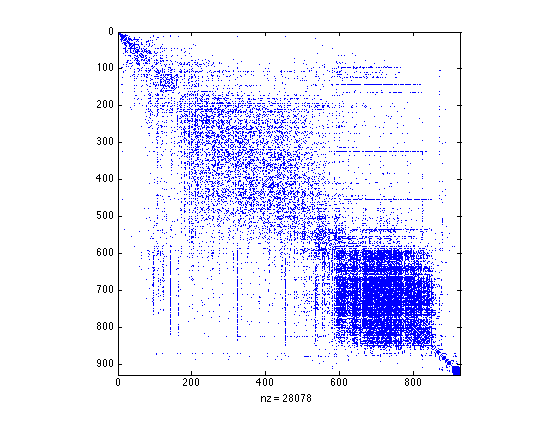
\includegraphics[ width=12cm,height=7cm]{fig1.png}
\caption{Sparsity plot of PageRank matrix P}
\label{fig1}
\end{figure}



%C
\problemAnswer{
\begin{enumerate}[(c)]
\item The following script calculates the normalized PageRanks and the tables dispay the top 5, for the unweighted case (top) and weighted case (bottom):
\end{enumerate}
}

\begin{verbatim}

% initialize values
alpha = .85;
v = ones(size(P,1),1) / size(P,1);

% Simple solve works in this case
pr = (eye(size(P,1)) - alpha*P)\v;

% normalize rank
pr = pr/norm(pr,1);

% sort and display top 5 ranked movies
[pr_sorted , sort_index] = sort(pr, 'descend');

for i= 1:5
    fprintf(1, '%f = %s (%s)\n', ...
    pr_sorted(i), movieName{sort_index(i)}, movieIMDbID{sort_index(i)});
end

\end{verbatim}

\begin{centering}
\begin{tabular}{|c|c|c|}\hline
PageRank & Movie Name  & IMDb movie ID  \\\hline
0.003957 & Gandhi & 0083987 \\\hline
0.003806 & JFK & 0102138\\\hline
0.003501 & Mr. Smith Goes to Washington & 0031679 \\\hline
0.003382 & A Star Is Born & 0047522 \\\hline
0.003297 & Citizen Kane & 0033467  \\\hline
\end{tabular}
\end{centering}

\bigskip
%D
\problemAnswer{
\begin{enumerate}[(d)]
\item  Because we don�t know the actual solution $x^*$, we cannot calculate (and thus cannot use the error defined by the expression $x-x^*$. Instead, we need another notion of convergence. Recall from Assignment 5 that if a PageRank calculation converges, it converges to the correct value. Thus, we calculate $x^{(k+1)}-x^{(k)}$ and determine whether its norm tends to $0$. Actually, we must be concerned with the relative norm, and so, for a given tolerance $\epsilon$, our stopping criterion is written

\begin{equation*}
\text{STOP   when   } \frac{ \| x^{(k+1)}-x^{(k)} \|_1}{\| x^{(k+1)} \|�}  < \epsilon
\end{equation*}

The following script calculates the normalized PageRank via Jacobi iteration and associated plots:

\end{enumerate}
}


\begin{verbatim}
%% Jacobi PageRank iteration

maxiter = 1e4; % more than enough
tol = 1e-4; 
alpha =0.85;

% pre-allocate an array to keep track of step length and iteration
iter_alloc = zeros(maxiter ,1);
step_length = zeros(maxiter ,1);

% previous iterate
x_old = zeros(size(P,1),1);

for iter = 1: maxiter
    
     	% next iterate
     	x_new = alpha*P*x_old + v;

     	% calculate convergenc measure
     	step_length(iter) = norm(x_new - x_old ,1)/norm(x_new ,1);

     	iter_alloc(iter) = iter;

     	if step_length(iter) < tol
     	     	break % convergence achieved! end
     	end
    
     	% update old iterate to current iterate
     	x_old = x_new;
    
end

% delete ununsed allocation
step_length = step_length(1:iter);
iter_alloc = iter_alloc(1:iter);

% normalize each solution and compare
x_new = x_new/norm(x_new ,1);

fprintf(1, 'Terminated in %d steps; normed difference in solutions is %f\n',...
iter, norm(x_new - pr))

% create plots
subplot(2,1,1), plot(iter_alloc , step_length)
title('Convergence per iterate , linear scale'); subplot(2,1,2), semilogy(iter_alloc , step_length)
title('Convergence per iterate, log-linear scale')
\end{verbatim}

\begin{figure}[h!]
\centering
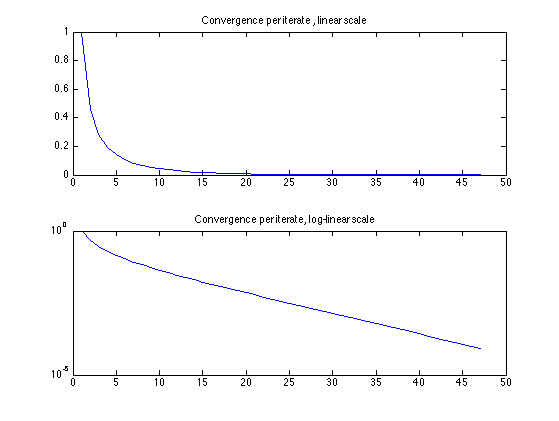
\includegraphics[ width=12cm,height=7cm]{fig2.png}
\caption{Convergence measure per iterate; shown in linear scale (top) and log-linear scale (bottom). My Jacobi iteration converged in 47 steps.
}
\label{fig2}
\end{figure}




%E
\problemAnswer{
\begin{enumerate}[(d)]
\item The following script plots rating and votes vs. PageRank:
\end{enumerate}
}

\begin{verbatim}
%% Plots

% PageRank vs. # of votes
subplot(2,1,1), plot(pr, movieVotes , 'b.');
title('PageRank vs. # of Votes')

% PageRank vs. movie rating
subplot(2,1,2), plot(pr, movieRating , 'b.');
title('PageRank vs movie rating')
\end{verbatim}

\begin{figure}[h!]
\centering
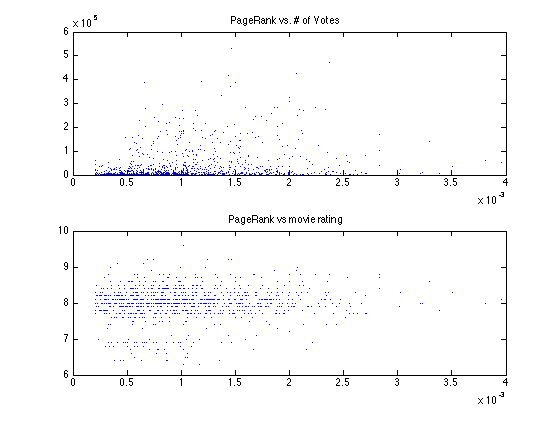
\includegraphics[ width=12cm,height=7cm]{fig3.png}
\caption{(Top) Votes versus PageRank; (Bottom) Rating vs. PageRank; note that for these measures, PageRank does not seem to be a very good indicator.
}
\label{fig3}
\end{figure}



\end{homeworkProblem}




\newpage





% Problem 2
\begin{homeworkProblem} 
Least squares (35 points)
We measured the temperature T below the ground on an unusually cold day a few weeks ago. The
temperature was measured as a function of the distance from the ground surface. The outside
temperature was a balmy 2 deg. Celsius. The data from the measurements are given in the table
below:

\begin{centering}
\begin{tabular}{|c|c|}\hline
Distance (m)  & Temperature (C) \\\hline
0 & 2.0 \\
5 & 2.2 \\
10 & 5.8 \\
15 & 10.4 \\
20 & 11.0 \\
25 & 13.8 \\
30 & 22.4 \\
35 & 28.4 \\
40 & 33.3 \\\hline
\end{tabular}

\end{centering}

\begin{enumerate}[(a)]
\item (15 points)
Write a matlab function that fits the data to a polynomial of degree $n$ using the method of
least squares.
Make sure that your function allows you to specify $n$. (Do not use matlab built-in functions
\texttt{polyfit} or \texttt{polyval} except perhaps to check that your code is correct.)
Plot the data. On the same axes, plot the polynomial fit for $n = 1$ and $n = 2$. Be sure to
clearly label your fit curves.

\item (10 points)
Calculate the residual error in your fitted values and the observed data for $n$ ranging from 0 to 8.

Plot the 2-norm of this residual error against $n$.

Comment on what does this result says about how to choose the order of your polynomial fit.

\item (10 points)
We improve our drilling and sensing methodology and decide that we can drill to 45m and 50m below ground with minimal efort. We want to estimate the temperature at this new data point.

\begin{enumerate}[(i)]
\item Provide a table of $n$ versus the predicted temperature at these new data points.
It turns out that the temperatures are 48.9 deg. Celsius at 45m and 57.9 deg. Celsius at 50m below ground, respectively.

\item Plot the 2-norm of the prediction error only at these two points versus $n$.

\item Comment on what does this result says about how to choose the order of your polynomial fit? Be sure to use what you learned from the previous problem.



\end{enumerate}
\end{enumerate}


\problemAnswer{
\begin{enumerate}[(a)]
\item We have a collection of points $\{(x_i, y_i)\}_{i=1}^K$ and want to fit an nth order polynomial to this data. That is, we want to find parameters $\beta_0, \beta_1, \dots, \beta_n$ such that


\begin{equation*}
\begin{split}
& y_1 = \beta_0 + \beta_1x_1 + \beta_2x_1^2 + \dots + \beta_n x_1^n + \epsilon_1 \\
& \hdots \\
& y_K = \beta_0 + \beta_1x_K + \beta_2x_K^2 + \dots + \beta_n x_K^n + \epsilon_K,
\end{split}
\end{equation*}

 where $\epsilon_i$ is the error in fit in the $i^{th}$ coordinate.

Defining the vector $y \in \mathbb{R}^K$ of response values, the vector $\beta \in \mathbb{R}^{n+1}$ of polynomial
coefficients, the vector $\vec \epsilon$ of errors and the �data matrix� $X \in \mathbb{R}^{K \times (n+1)}$ defined by
$X_{ij} = x_i^{j-1}$, we can write this as a matrix system, 

\begin{equation*}
\vec y = X \vec \beta + \vec \epsilon
\end{equation*}

That is, we want to find the coefficients $\beta^*$ that define the polynomial minimizing the
squared error  $\| \vec \epsilon\|_2$, which we can compute via the normal equations $X^T \vec y = X^T X \vec \beta^*$. Perhaps best for us, matlab�s backslash operator gives us the solution to the normal
equations. Thus the following function gives the polynomial coefficients of best fit $\beta^*$:





\end{enumerate}
}

\begin{verbatim}
function [ beta ] = mypolyfit (x , y , n)

% Fits an n-th order polynomial to pairs (x(i), y(i)) 
% Returns the coefficients beta 0 , beta 1 , ... , beta n 
% for P(x) = beta 0 + beta 1 x + ... + beta n x^n
% minimizing sum[ (y i - P(x i))^2 ]


% Turn inputs into column vectors
myx = x ( : ); 
myy = y ( : ) ;

K= size(myx,1);

% % One way to construct the data matrix % X = zeros(K, n+1);
%
% % Using for loops
%for p=0:n, 
%X(:,p+1)=myx .^p; 
% end


% Construct the data matrix
X= repmat(myx,[1,n+1]) .^ kron(ones(K,1), 0:n); 


% Return the least squares solution
beta = X \ myy; 
end
\end{verbatim}

\problemAnswer{ Then the following function gives the polynomial defined by the coefficients $\beta_i$ at the points $x_i$ :}

\begin{verbatim}
function [yhat] = mypolyval(x, beta)
% Takes a collection of x values and betas definining a
% polynomial and calculates 
% yi=P(xi)=beta0+beta1 xi+...+betan xi�n

% Turn inputs into column vectors
mybeta = beta(:); 
myx = x ( : ) ;

n = size(mybeta,1)-1; % order of polynomial

p=size(myx,1); %number of x points 

% Construct the data matrix
X= repmat(myx,[1,n+1]).^kron(ones(p,1), 0:n); 

yhat = X*mybeta;

end\end{verbatim}

\problemAnswer{And the following program uses the above two functions to calculate the linear and quadratic polynomial fits to our data, plotting it all on one set of axes with a legend:}

\begin{verbatim}
dist = (0:5:40)';
temp = [2; 2.2; 5.8; 10.4; 11.0; 13.8; 22.4; 28.4; 33.3];

beta1 = mypolyfit ( dist , temp ,1);
beta2 = mypolyfit ( dist , temp , 2);

plot(dist, temp, 'k.'); 
hold on ;

x = linspace (0 ,40 ,100) ; 
plot(x, mypolyval(x, beta1) ,'g-') ;
plot(x, mypolyval(x, beta2) ,'b-');

legend('Given data','Linear fit ','Quadratic fit ', 'Location','NorthWest');
\end{verbatim}

\problemAnswer{
The polynomial fits of first and second order are plotted along with the data in the following figure:}

\begin{figure}[h!]
\centering
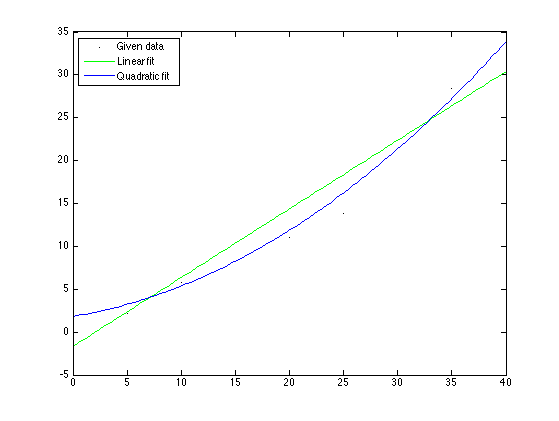
\includegraphics[ width=12cm,height=7cm]{fig4.png}
\caption{Our fitted temperature data.
}
\label{fig4}
\end{figure}



\problemAnswer{
\begin{enumerate}[(b)] \item  The following code calculates the residual error as the polynomial order n changes from 0 to 8: \end{enumerate}}

\begin{verbatim}
% Create a function to compute the 2-norm of the residual as defined by n 
resid = @(n) norm(temp - mypolyval(dist , mypolyfit(dist , temp, n)));

% Compute this function for n = 0:8
error_n = arrayfun(resid , 0:8);

plot (0:8 , error_n ) ;
xlabel( ' Order of polynomial ' ) ; 
ylabel('Residual 2-norm');
\end{verbatim}

\problemAnswer{The (in-sample) error plot is given in the following figure: }


\begin{figure}[h!]
\centering
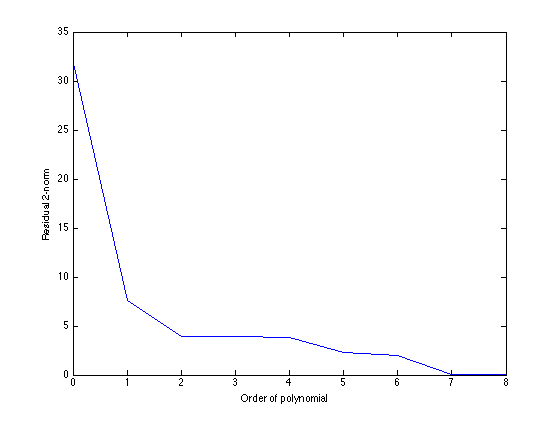
\includegraphics[ width=12cm,height=7cm]{fig5.png}
\caption{(In-sample) error versus order of polynomial fit.
}
\label{fig5}
\end{figure}


\problemAnswer{ The graph above suggests we want to fit the highest order polynomial to our data in order to reduce our fitted (in-sample) error as much as possible. Note that k points uniquely define a polynomial of order k - 1, thus the error when $n = 8$ is 0. This also means that it would not make sense to use an $n > 8$ since $n=8$ already fit the data points.}




\problemAnswer{
\begin{enumerate}[(c)] \item The following program calculates the predicted values at the new data points, then calculates the residual and its 2-norm for values of n from 0 to 8: \end{enumerate}}

\begin{verbatim}
newdist = [45; 50]; 
newtemp = [48.9; 57.9];

% Create a function to compute the predicted values
predict = @(n) mypolyval ( newdist , mypolyfit ( dist , temp , n) ) ;

% Calculate the predicted values for varying n
predicted = zeros(2 ,9) ; 
for n = 0:8
	predicted(:,n+1) = predict(n);
end

% Create a function to compute the 2-norm of the predicted error
resid =@(n) norm(newtemp- mypolyval(newdist, mypolyfit(dist, temp, n)));

% Compute this function for n = 0:8
error_n = arrayfun(resid , 0:8)

alldist = [ dist ; newdist ]; 
alltemp = [temp; newtemp];

% Create a function to compute the 2-norm of the total error
resid = @(n) norm(alltemp-mypolyval(alldist , mypolyfit(dist , temp, n)));

% Compute this function for n = 0:8
error_n = arrayfun(resid , 0:8)
semilogy(0:8 , error_n ) ;
xlabel ( ' Order of polynomial ') ; 
ylabel('Total error residual 2-norm');
\end{verbatim}

\problemAnswer{The results are tabulated as follows:}


\begin{centering}
\begin{tabular}{|c|c c|c|}\hline
actual & 48.9000 & 57.9000 & -  \\\hline \hline
model & $\hat y$(45m) &  $\hat y$(50m) &   \\\hline \hline
n = 0 & 14.3667 &  14.3667 &  55.5671  \\\hline
n = 1 &    34.4000  & 38.4067  &  24.2949  \\\hline
n = 2 &    41.2571 &  49.3781 &   11.4471\\\hline
n = 3 &    41.7238 &  50.4048  & 10.3767\\\hline
n = 4 &    38.6667  & 41.2333  & 19.5576\\\hline
n = 5 &    18.5000 & -39.4333 & 101.9703\\\hline
n = 6 &    34.9667  & 46.1933  & 18.1985 \\\hline
n = 7 &   133.1333 &  694.0933 &  641.745440  \\\hline
n = 8 &   123.5000   &  615.1000 &  562.1717 \\\hline
\end{tabular}
\end{centering}

  
  
\problemAnswer{This suggests that the previous result may not be accurate, i.e. that we may not always want to choose n as large as possible as we may be �overfitting� our model to our data. In fact, this out-of-sample error grows after n grows large.
If we calculate the total residual error (fitted �in-sample� error plus predicted �out-of- sample� error), we get the following very informative plot in Figure 7.
Thus we may be best off fitting this data to a cubic polynomial. Funnily enough, the data were constructed by the following matlab command, defining a quadratic polynomial and adding random noise with standard deviation 3:}

\begin{verbatim}
temp = 0.6 *(dist/5) .^ 2 - 0.5 * (dist/5) + 2 + 3 * randn(size(dist))
\end{verbatim}

\begin{figure}[h!]
\centering
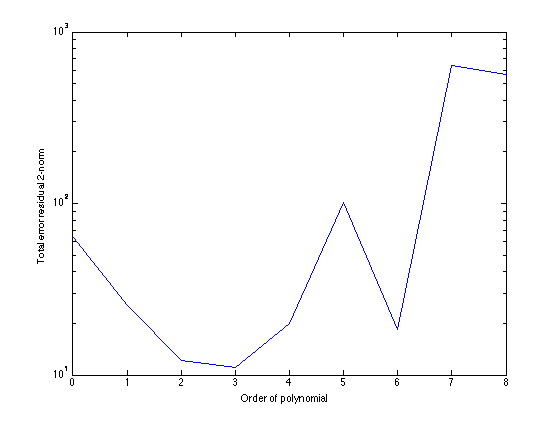
\includegraphics[ width=12cm,height=7cm]{fig6.png}
\caption{Total (in-sample + out-of-sample) error versus order of polynomial fit.
}
\label{fig6}
\end{figure}

\end{homeworkProblem}
  
  
\end{document}
 
 
 
